%%%%%%%%%%%%%%%%%%%%%%%%%%%%%%%%%%%%%%%%%%%%%%%%%%%%%%%%%%%%%%%%%%%%%%%%
% Plantilla TFG/TFM
% Escuela Politécnica Superior de la Universidad de Alicante
% Realizado por: Jose Manuel Requena Plens
% Contacto: info@jmrplens.com / Telegram:@jmrplens
%%%%%%%%%%%%%%%%%%%%%%%%%%%%%%%%%%%%%%%%%%%%%%%%%%%%%%%%%%%%%%%%%%%%%%%%

\chapter{Materials and Methods}
\label{metodologia}
In this chapter we will go through some of the software and hardware specification related to this work, making special emphasis in those we ended up using as our main resources. We will divide this chapter in 4 different parts. First, we needed a game or 3D engine framework in order to generate our synthetic data. Second, we needed a high level deep learning framework in order to implement some of the current architectures, since most of them are quite complex and building them from the ground up is a extremely complex task and out of the scope of this work. Third, we need real world datasets in order to test our synthetic data trained algorithms. And finally, we need extremely powerful GPU computing hardware in order to train and test these architectures.

\section{Unreal Engine 4}
\gls{ue4} is a very powerful, highly portable game engine, written in C++ and developed by Epic Games\footnote{\url{https://www.unrealengine.com/en-US/}}.
The main advantages \gls{ue4} offers over other game engines and the reason UnrealROX was built using it are listed as follows:

\begin{itemize}
	\item \textbf{Virtual reality support:} VR was a key point when developing the ROX framework since one of the main goals was to allow the user to completely interact with the environment.
	\item \textbf{Photorealism:} Realism is a key factor when it comes to synthetic data and \gls{ue4} potential to run extremely realistic scenes, such as the one shown in figure \ref{fig:london_apartment}, in real time made it perfect for this purpose.
	\item \textbf{Blueprints:} Blueprints are one of the tools that \gls{ue4} offers and it allows for quick behavior definitions in the editor without writing a single line of code. This makes it perfect for prototyping and testing.
	\item \textbf{Community:} \gls{ue4} is currently one of the most popular game engines and it has a rather big community, the official forums and other platforms are very active and the documentation is well maintained. The developing team is very active and they continuously release new versions and bug fixes. 
\end{itemize}

\begin{figure}[h]
	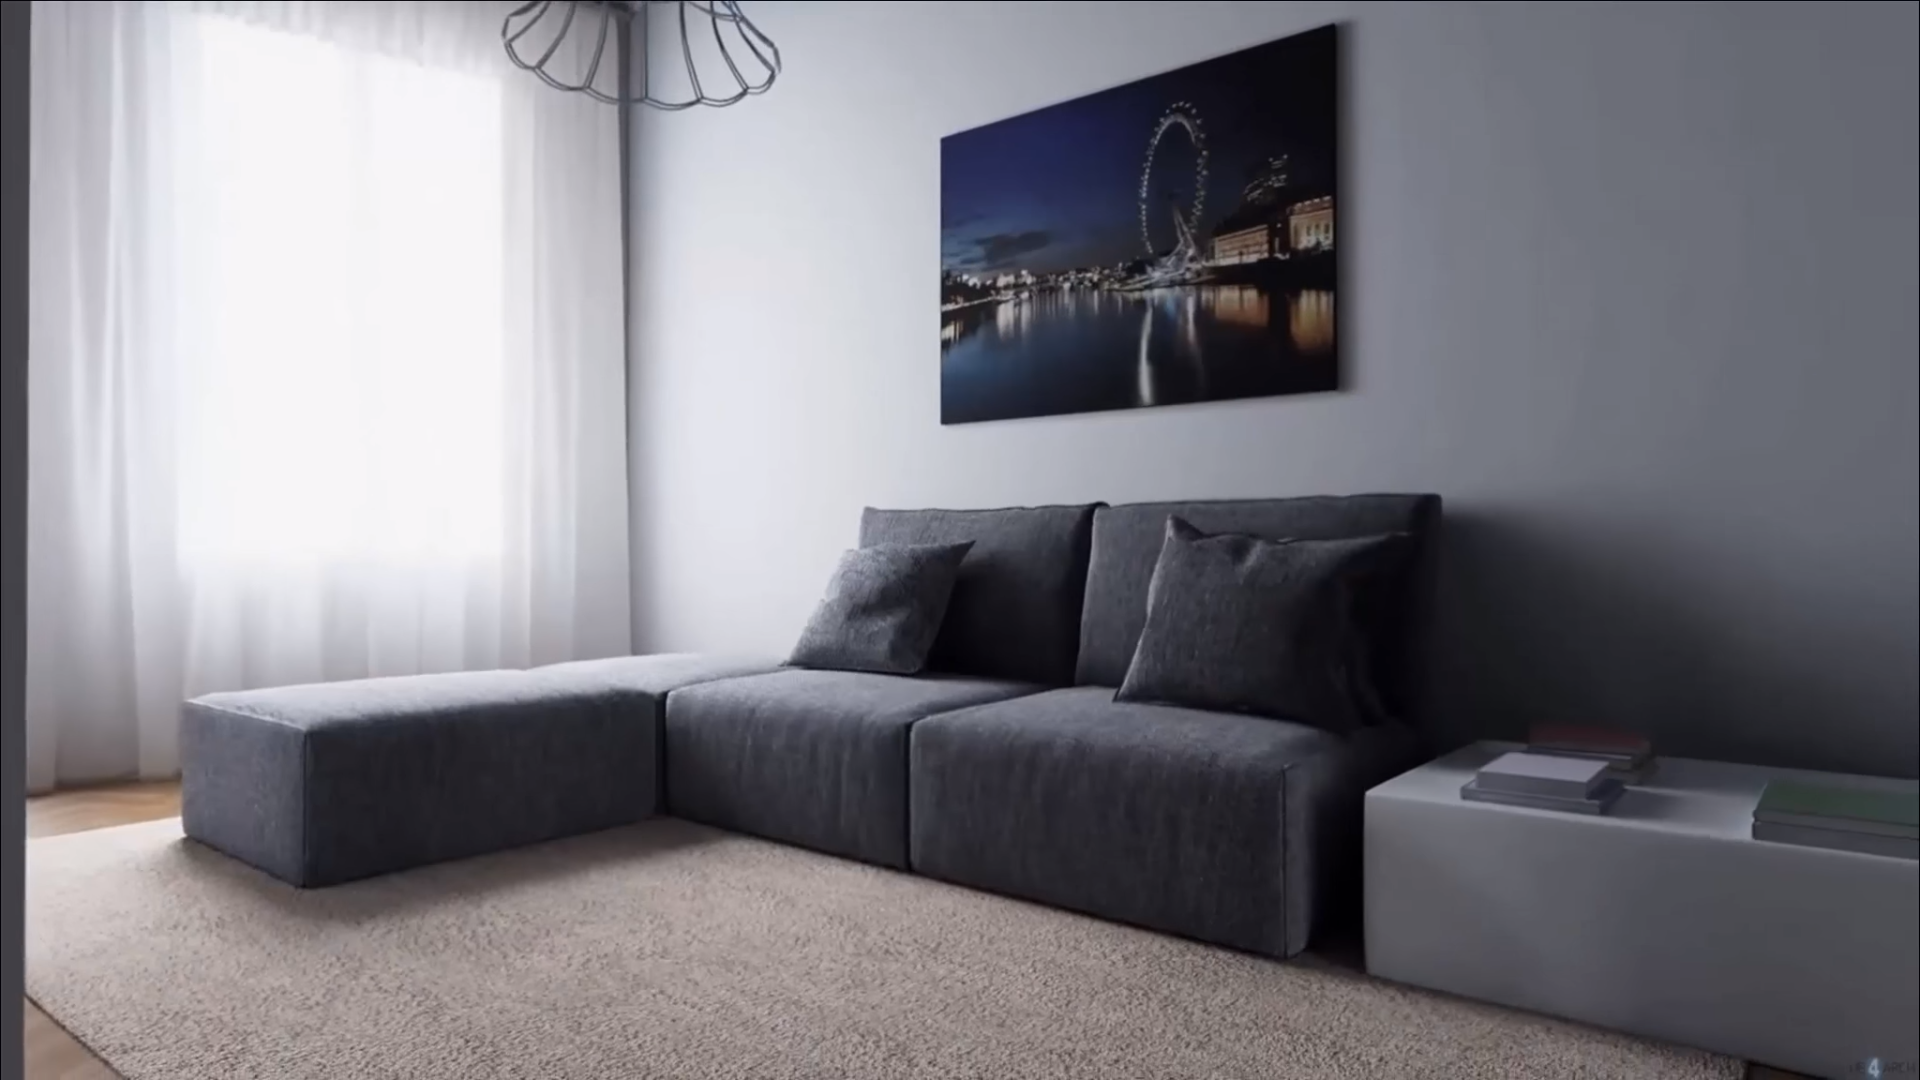
\includegraphics[scale=0.2]{archivos/london_apartment.png}
	\centering
	\caption[Snapshot of the Viennese Apartbent by UE4Arch]{Snapshot of the Viennese Apartment by UE4Arch\footnotemark}
	\label{fig:london_apartment}
\end{figure}
\footnotetext{\url{https://ue4arch.com/projects/viennese-apartment/}}

\section{Visual Studio 2017}
Visual Studio is an \gls{ide} developed by Microsoft and used for software development. It supports a variety of programming languages, although mainly focuses on C++, C\# and the .NET framework. It includes a code editor, file browser and debugger. It also includes plugins, support for syntax highlighting and comes integrated with IntelliSense, which allows for code completion, quick information of variables and methods, amongst others features.

However the main reason Visual Studio was chosen as the main \gls{ide} for this project is the integration with \gls{ue4}. The \gls{ue4} editor has options to quickly visualize any object from the context menu or the scene in Visual Studio, allowing to make quick changes, recompile and launch in very little time.

\begin{figure}[h]
	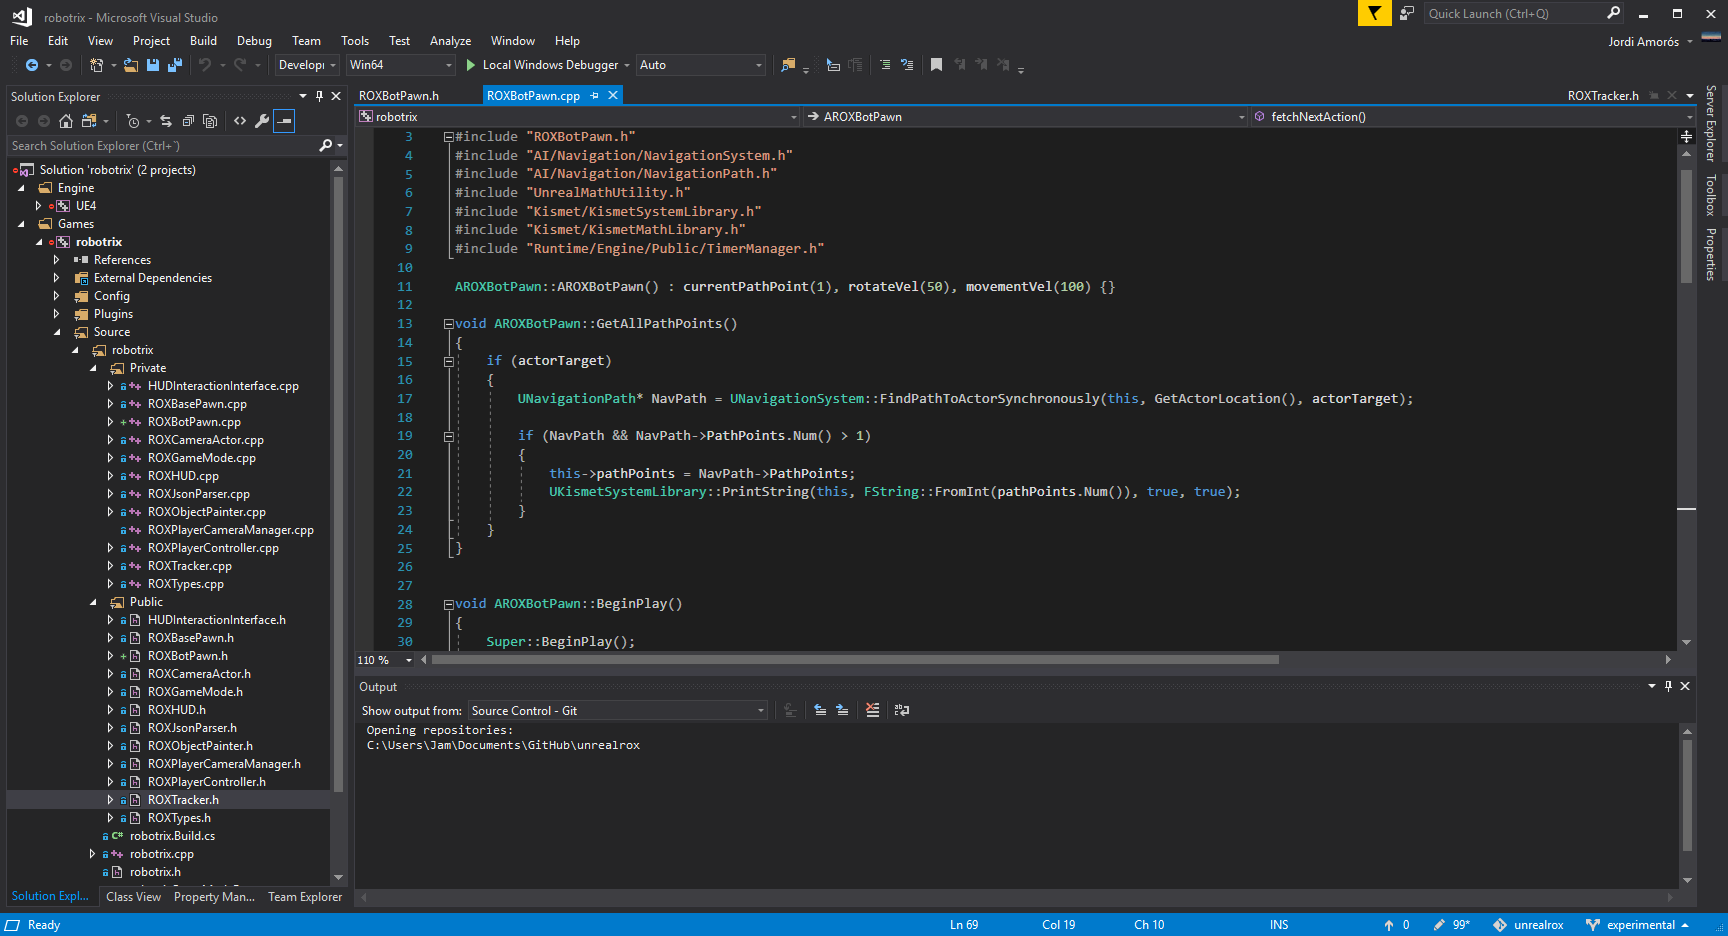
\includegraphics[width=0.7\textwidth]{archivos/vs_ide.png}
	\centering
	\caption{Visual Studio IDE.}
	\label{fig:visual_studio}
\end{figure}

\section{Frameworks}
In this section, we will go trough some of the most recent and popular \gls{dl} frameworks.

\subsection{TensorFlow}
TensorFlow is a open source library for numerical computation based on the idea of data flow graphs. In TensorFlow, the graph nodes represent the mathematical operations, while the edges represent the multidimensional data arrays (or tensors) flowing between them, Figure \ref{fig:tensorflow} illustrates an example of a flow graph representation.

\begin{figure}[h]
	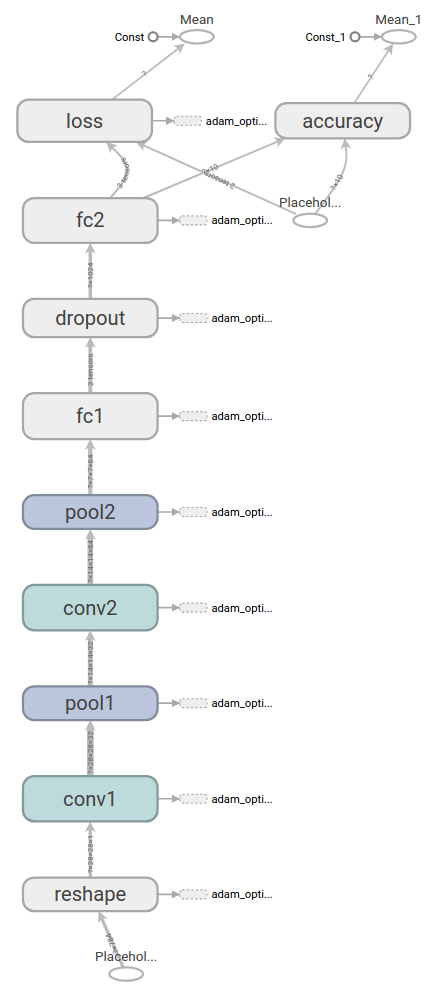
\includegraphics[scale=0.3]{archivos/tensorflow.png}
	\centering
	\caption{Tensorflow graph example depicting a simple two-layer convolution + pooling with a fully connected layer for classification at the end.}
	\label{fig:tensorflow}
\end{figure}

TensorFlow was created by the researches at Google Brain for the purpose of conducting machine learning and deep neural network research, its low level nature allows for a very fine-grained framework that can be use to build any architecture from the ground up and the tensor-graph structure also allows for very easy distribution on the CPU-GPU.

In a first approach, TensorFlow was going to be the main framework for this project, but was finally discarded since high level frameworks will ease the work and the low level implementation of the networks fall out of the scope of this project.

\subsection{Keras}
Keras is a high level framework written in Java that can use TensorFlow, CNTK or Theano as backend. It was developed to be an easy to use framework, allowing for very fast experimentation and prototyping, abstracting the user of some of the more complex low level tasks with a very user friendly interface. This also makes Keras a very good entry framework for beginners that still don't have a solid foundation on deep learning.

Keras provides two different APIs for different model building approaches. The Sequential API which allows to simply stack layer after layer, allowing for a very simple and easy to use interface for models with a input to output data flow. The Functional API however allows for more complex models by understanding each layer as a node graph, allowing for different, more complex and non sequential models.
 
\subsection{PyTorch}
PyTorch is an open source, Python-based, \gls{gpu}-Ready computing package and machine learning framework, just like other frameworks, it provides Tensors, which can be moved both to the \gls{cpu} and \gls{gpu}, as well as all the algebra and math operations for them, they can also be converted from NumPy and other Tensor libraries.

Another PyTorch feature that is worth mentioning is the modularity, writing new modules for a \gls{nn} is very straightforward and they can be written in both native python and other NumPy based libraries or with the torch \gls{api}.

PyTorch is also in continuous development and has been steadily gaining popularity ever since its release back in 2016. In terms of performance, PyTorch is just slightly behind Tensorflow, and easily outperforms other high level frameworks such as Keras.

\begin{figure}[h]
	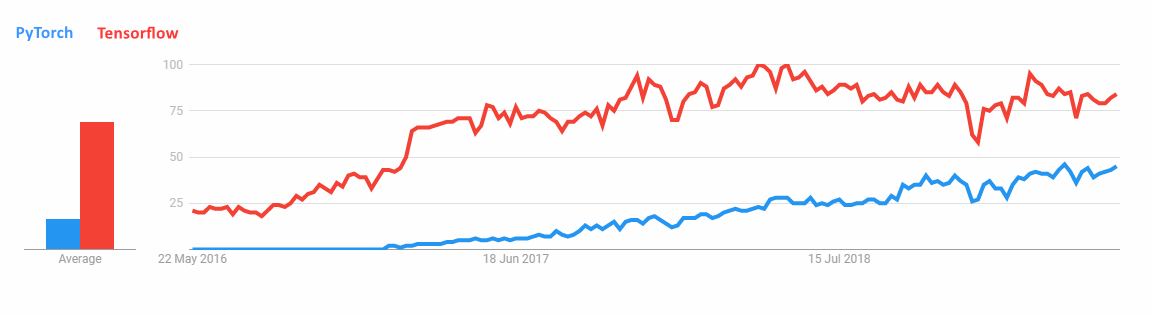
\includegraphics[width=\textwidth]{archivos/pytorch.png}
	\centering
	\caption{Worldwide PyTorch and Tensorflow popularity comparison in Google Search.}
	\label{fig:pytorch}
\end{figure}

PyTorch was the framework of choice for this project since it allows for easy prototyping without losing the flexibility to make architectural modifications to the networks. Its syntax is also very easy for anyone that has experience with python which made it perfect for this project.

\section{Hardware}
It is widely known how computationally demanding \gls{dl} algorithms are, specially when dealing with large amounts of data. Also, in order to smoothly run \gls{ue4} while recording and generating all the output images we need a mid to high end computer. In this section we review the ones that have been mainly used in this work.

\subsection{Asimov}

The structure of neural networks where multiple data streams are organized in layers allow for very easy paralelization. Because of this GPU's are extremely powerful when executing said algorithms.

The Asimov server was deployed with this in mind and features three different NVIDIA GPUs. The most powerful of them, the Titan X is aimed towards \gls{dl} computing, the Tesla K40 is also used for computational purposes. The last of them is a GTX 730 that will only be used for visualization purposes. The full hardware specification for the Asimov server is shown in Figure \ref{table:asimov}.

As for the software, Asimov runs Ubuntu 16.04 with Linux kernel 4.4.0-21-generic for x86\_64 architecture. It also runs Docker, which allows any user to configure its own container with any CUDA / CUDNN version and DL framework.

Also, it is worth mentioning  Asimov was configured for remote access using SSH with public/private key pair authentication. The installed versions are OpenSSH 7.2p2 with OpenSSL 1.0.2 and X11 forwarding was configured for visualization purposes.

\begin{table}[h]
	\centering 
	\begin{tabular}{c p{7cm}}
		\hline
		\multicolumn{2}{c}{Asimov} \\ [0.5ex] 
		\hline
		Motherboard & Asus X99-A \newline Intel X99 Chipset \newline 4x PCIe 3.0/2.0 x 16(x16, x16/ x16, x16/ x16/ x8) \\ 
		\hline
		CPU & Intel(R) Core(TM) i7-5820K CPU @ 3.3GHz \newline 3.3 GHz (3.6 GHz Turbo Boost) \newline 6 cores (12 threads) \newline 65 W TDP \\
		\hline
		GPU (visualization) & NVIDIA GeForce GT730 \newline 96 CUDA cores \newline 1024 MiB of DDR3 Video Memory \newline PCIe 2.0 \newline 49 W TDP \\
		\hline
		GPU (deep learning) & NVIDIA GeForce Titan X \newline 3072 CUDA cores \newline 12 GiB of GDDR5 Video Memory \newline PCIe 3.0 \newline 250 W TDP\\
		\hline
		GPU (compute) & NVIDIA Tesla K40c \newline 2880 CUDA cores \newline 12 GiB of GDDR5 Video Memory \newline PCIe 3.0 \newline 235 W TDP \\
		\hline
		RAM & 4 x 8 GiB Kingston Hyper X DDR4 2666 MHz CL13 \\
		\hline
		Storage (Data) & (RAID1) Seagate Barracuda 7200rpm 3TiB SATA III HDD \\
		\hline
		Storage (OS) & Samsung 850 EVO 500GiB SATA III SSD \\
		\hline
	\end{tabular}
	\caption{Hardware specification for Asimov.}
	\label{table:asimov}
\end{table}

\subsection{Personal Computer}
During the developing of this work, my personal computer was used in order to run \gls{ue4} and UnrealROX, as well as generating the data used for the deep learning experimentation. Table \ref{table:pc} shows the full hardware specification.

\begin{table}[h]
	\centering 
	\begin{tabular}{c p{7cm}}
		\hline
		\multicolumn{2}{c}{Personal Computer} \\ [0.5ex] 
		\hline
		Motherboard & Asus STRIX X370-F \newline Amd X370 Chipset \newline 2 x PCIe 3.0/2.0 x16 (x16 or dual x8)  \\ 
		\hline
		CPU & AMD Ryzen™ 5 1600 CPU @ 3.2GHz \newline 3.2 GHz (3.6 GHz Turbo Boost) \newline 6 cores (12 threads) \newline 140 W TDP \\
		\hline
		GPU & NVIDIA GeForce GTX960 \newline 1024 CUDA cores \newline 2048 MiB of DDR5 Video Memory \newline PCIe 3.0 \newline 120 W TDP \\
		\hline
		RAM & 2 x 8 GiB G.Skill Trident Z DDR4 3200 MHz CL15 \\
		\hline
		Storage (Data) & Seagate Barracuda 7200rpm 2TiB SATA HDD \\
		\hline
		Storage (OS) & Samsung 960 EVO 250GiB NVMe M.2 SSD \\
		\hline

	\end{tabular}
	\caption{Hardware specification for my personal computer.}
	\label{table:pc}
\end{table}
